Different methods of software development exist in software engineering. It is important to choose a proper development process before a team starts developing. Different types of development processes mean a different way of testing. This chapter explains the development methods and how to organise performance regression testing when using each of these methods.

\section{Code-and-fix model}
The code-and-fix model was the model used in the early days of software development. It contained only two steps: write some code and fix the problems in the code \cite{boehm1988spiral}. This method is not appropriate for performance regression testing, because of the poor preparation of the testing process. It is hard to write test suites without a plan and knowledge of the overall design, especially if there is none.

\section{Waterfall method}
The waterfall method establishes a sequence of stages to guid the development process: requirements, specifications, design, coding, testing and maintenance \cite{kang1989software}. The sequences of the waterfall method will be repeated until the development of the system is completed. The waterfall method even became the basis for most software acquisition standards in past years \cite{boehm1988spiral}. Figure \ref{Figure:Waterfall} gives the phases of the waterfall method.

\begin{figure}[H]
\label{Figure:Waterfall}
\begin{center}
  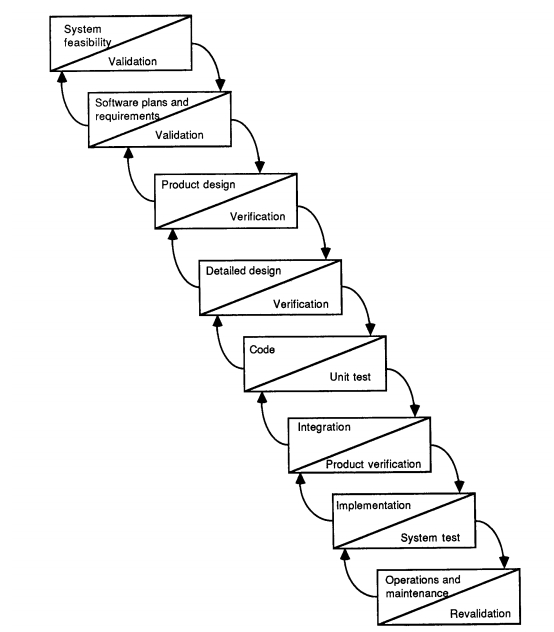
\includegraphics[width=0.5\textwidth]{Figures/waterfall.jpg}
\end{center}
  \caption{Different development phases of the waterfall method \cite{boehm1988spiral}.} 
\end{figure}

Each rectangle in Figure \ref{Figure:Waterfall} states a phase in the waterfall development process. When an error occurs the current state will be checked first, then the previous states will be checked until the cause of the error is found. The waterfall method is a static development process, meaning that when the process is done, the product is finished. The testing is done near the end of the process, which means that performance regressions are tested near the end of the process too. This suggests that performance regression testing will not be effective, because the tests will be executed when the implementation is (almost) done. Unfortunately, it has been stated that most of the time performance is the biggest issue in the field \cite{foo2010mining}. Luckily, when using an iterative form of the waterfall method, it can be tested more effectively. Collins et al. studied an agile waterfall process \cite{collins2010iterative}. This research showed that when using an iterative process, regression testing using the waterfall method can be very useful. The combination of performance as biggest issue and an effective way of regression testing when using an iterative waterfall process suggests that performance regression testing can be done effective here too.

\section{Spiral method}
The spiral method creates a risk-driven approach to the software process rather than a primarily document-driven or code-driven approach. It incorporates many of the strengths
of other models and resolves many of their
difficulties\cite{boehm1988spiral}. The phases of the spiral development process are shown in Figure \ref{Figure:Spiral}. 

\begin{figure}[H]
\label{Figure:Spiral}
\begin{center}
  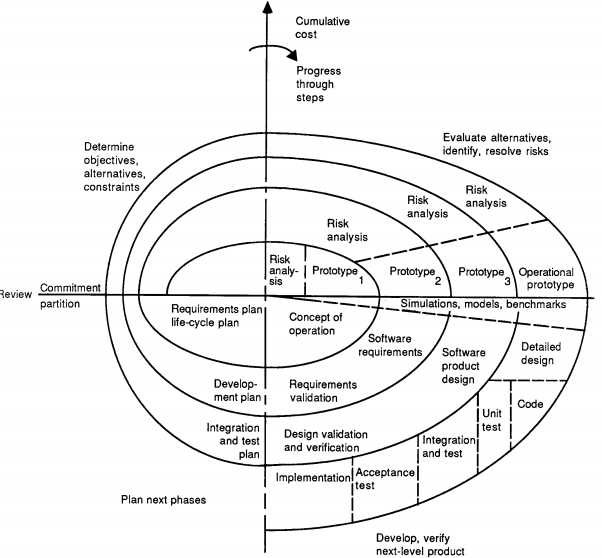
\includegraphics[width=0.5\textwidth]{Figures/spiral.jpg}
\end{center}
  \caption{Different development phases of the spiral method \cite{boehm1988spiral}.} 
\end{figure}

When using the spiral model, the main focus lies on the different risks of a software project. Examples of these risks are: a low budget, a wrong approach to development and continously changing code. The spiral development process has a phase for each risk. Different prototypes will be made implementing a solution to the risks. Performance regressions can be seen as a risk too, because it can be a demand to maintain the performance of the prototypes. This means that the performance regression testing can be effectively organised when using the spiral method.

\section{Scrum}
Scrum is an agile software development process designed to add energy, focus, clarity, and transparency to development teams \cite{sutherland2007distributed}. Scrum is divided into three phases. There are two organising phases, which are the opening and closing phases, and an implementing phase. The implementing phase is further divided into sprints. The planning and closing phases are organising phases. It is not necessary to run tests here, because there is either no code (opening) or all the performance regression tests have been executed and passed (closing). Though, examples of organising aspects which can be done during the opening and closing phases are planning when to test and verifying that the test suite covers all the code. \\ The actual creation of tests will be done during the sprints. The sprints consist of developing, wrapping, reviewing and adjusting. The wrapping part of the sprint combines all the implemented code. This process of wrapping is a very appropriate moment to test for performance regressions. \\ Research has been done to show that automated regression tests during the sprints will greatly improve the quality of the product \cite{Future_of_Scrum}. This means that Scrum is a useful development method for regression testing. When the performance is monitored here as well, the combination of the two can make the testing of performance regressions effective.  \\ 

\section{General aspects of test organization}
Despite the fact that the development method is significant, there are some other organising aspects which could make a difference in the way of performance regression testing. \\
First of all, it can be important who will do the testing. If the testing is done by one person it can be effective. This person is an active member of the team and watches all the members of the development team. This method provides a way to deal with any issues that could come up during the process. The appointed person will try to directly deal with these issues. By appointing this person, the quality of the product is monitored the whole time during the project, as opposed to the alternative research where the testing is done by the team.  Sutherland et al. performed an experiment in which one person did all the testing throughout the project \cite{sutherland2009fully}. This experiment indicated that the quality of the development got a much higher average score compared to other similar development products. So appointing one tester who only has the task to watch over the quality by testing, and in the context of this report performing regression tests, can have an improved effect on the overall process. It is not mandatory to use this role division, but it can have a great impact on the performance of the overall product. \\

Another organising aspect is to make sure a proper test suite is  written and maintained. Test suites should be made with some conditions in mind. Writing complete test suites for complex systems will require the regression testing to run for a long time \cite{rothermel2001prioritizing}. So the developers have to decide to either test the complete system or write selective test suites. These selective test suites will only test the main functionality of the system. \\
After the organising phase, the actual implementation will be initiated. From now on the test suite will be actived and the test results will have to be processed in order to detect performance regressions. In order what know what to do with these results, we first need to know what kind of results we can expect. 
